\documentclass[12pt,fleqn]{article}\usepackage[]{graphicx}\usepackage[]{color}
%% maxwidth is the original width if it is less than linewidth
%% otherwise use linewidth (to make sure the graphics do not exceed the margin)
\makeatletter
\def\maxwidth{ %
  \ifdim\Gin@nat@width>\linewidth
    \linewidth
  \else
    \Gin@nat@width
  \fi
}
\makeatother

\definecolor{fgcolor}{rgb}{0.345, 0.345, 0.345}
\newcommand{\hlnum}[1]{\textcolor[rgb]{0.686,0.059,0.569}{#1}}%
\newcommand{\hlstr}[1]{\textcolor[rgb]{0.192,0.494,0.8}{#1}}%
\newcommand{\hlcom}[1]{\textcolor[rgb]{0.678,0.584,0.686}{\textit{#1}}}%
\newcommand{\hlopt}[1]{\textcolor[rgb]{0,0,0}{#1}}%
\newcommand{\hlstd}[1]{\textcolor[rgb]{0.345,0.345,0.345}{#1}}%
\newcommand{\hlkwa}[1]{\textcolor[rgb]{0.161,0.373,0.58}{\textbf{#1}}}%
\newcommand{\hlkwb}[1]{\textcolor[rgb]{0.69,0.353,0.396}{#1}}%
\newcommand{\hlkwc}[1]{\textcolor[rgb]{0.333,0.667,0.333}{#1}}%
\newcommand{\hlkwd}[1]{\textcolor[rgb]{0.737,0.353,0.396}{\textbf{#1}}}%
\let\hlipl\hlkwb

\usepackage{framed}
\makeatletter
\newenvironment{kframe}{%
 \def\at@end@of@kframe{}%
 \ifinner\ifhmode%
  \def\at@end@of@kframe{\end{minipage}}%
  \begin{minipage}{\columnwidth}%
 \fi\fi%
 \def\FrameCommand##1{\hskip\@totalleftmargin \hskip-\fboxsep
 \colorbox{shadecolor}{##1}\hskip-\fboxsep
     % There is no \\@totalrightmargin, so:
     \hskip-\linewidth \hskip-\@totalleftmargin \hskip\columnwidth}%
 \MakeFramed {\advance\hsize-\width
   \@totalleftmargin\z@ \linewidth\hsize
   \@setminipage}}%
 {\par\unskip\endMakeFramed%
 \at@end@of@kframe}
\makeatother

\definecolor{shadecolor}{rgb}{.97, .97, .97}
\definecolor{messagecolor}{rgb}{0, 0, 0}
\definecolor{warningcolor}{rgb}{1, 0, 1}
\definecolor{errorcolor}{rgb}{1, 0, 0}
\newenvironment{knitrout}{}{} % an empty environment to be redefined in TeX

\usepackage{alltt}
\usepackage{pgfplots}
\pgfplotsset{compat=1.7}
\usepackage{graphicx}
\usepackage[margin=1in]{geometry} 
\usepackage{amsmath,amsthm,amssymb,scrextend}
\usepackage{fancyhdr}
\pagestyle{fancy}
\DeclareMathOperator{\rng}{Rng}
\DeclareMathOperator{\dom}{Dom}
\newcommand{\R}{\mathbb R}
\newcommand{\cont}{\subseteq}
\newcommand{\N}{\mathbb N}
\newcommand{\Z}{\mathbb Z}
\usepackage{tikz}
\usepackage{pgfplots}
\usepackage{amsmath}
\usepackage[mathscr]{euscript}
\let\euscr\mathscr \let\mathscr\relax% just so we can load this and rsfs
\usepackage[scr]{rsfso}
\usepackage{amsthm}
\usepackage{amssymb}
\usepackage{multicol}
\usepackage[colorlinks=true, pdfstartview=FitV, linkcolor=blue,
citecolor=blue, urlcolor=blue]{hyperref}

\DeclareMathOperator{\arcsec}{arcsec}
\DeclareMathOperator{\arccot}{arccot}
\DeclareMathOperator{\arccsc}{arccsc}
\newcommand{\ddx}{\frac{d}{dx}}
\newcommand{\dfdx}{\frac{df}{dx}}
\newcommand{\ddxp}[1]{\frac{d}{dx}\left( #1 \right)}
\newcommand{\dydx}{\frac{dy}{dx}}
\let\ds\displaystyle
\newcommand{\intx}[1]{\int #1 \, dx}
\newcommand{\intt}[1]{\int #1 \, dt}
\newcommand{\defint}[3]{\int_{#1}^{#2} #3 \, dx}
\newcommand{\imp}{\Rightarrow}
\newcommand{\un}{\cup}
\newcommand{\inter}{\cap}
\newcommand{\ps}{\mathscr{P}}
\newcommand{\set}[1]{\left\{ #1 \right\}}

\renewcommand{\labelenumi}{(\alph{enumi})} %first level: (a),(b)
\renewcommand{\labelenumii}{\roman{enumii}.} %second level: i,ii

\theoremstyle{definition}
\newtheorem*{sol}{Solution}
\newtheorem*{claim}{Claim}
\newtheorem{problem}{}
% ---------------------------------------------------------------------------------------------
\IfFileExists{upquote.sty}{\usepackage{upquote}}{}
\begin{document}
\lhead{Machine Learning}
\chead{Zhijian Liu}
\rhead{\today}



% Just put your proofs in between the \begin{proof} and the \end{proof} statements!

\section*{Homework \#2}
% 1.
	\begin{problem} (\#3-1, page 120).The following table contains results of linear regression analysis of \textit{Advertising data}. It was used to model number of units sold as a function of radio, TV, and newspaper advertising budgets.
	  \begin{figure}[h!]
	  \centering
	    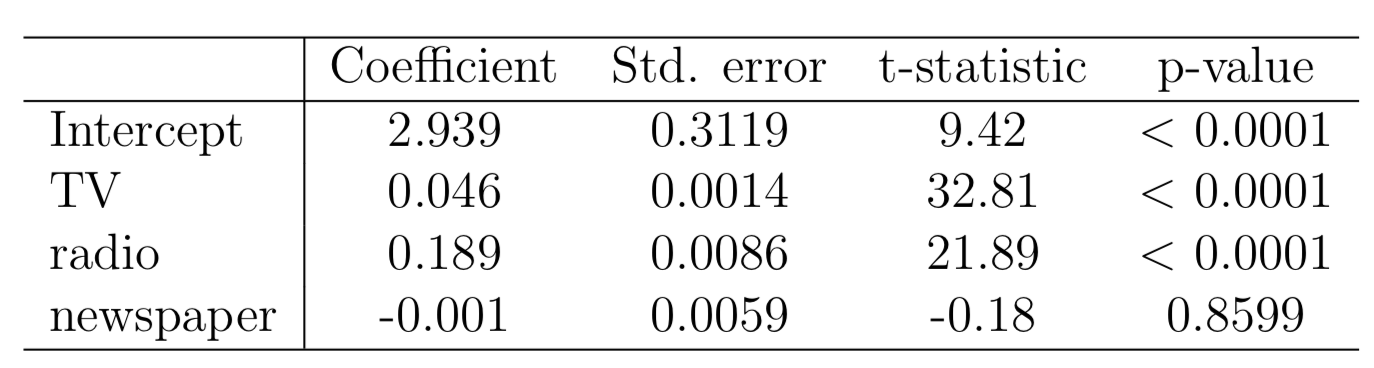
\includegraphics[width=0.65\linewidth]{chart.png}
	  \end{figure}
	  Describe the null hypotheses to which the given p-values correspond. Explain what conclusions you can draw based on these p-values. Your explanation should be phrased in terms of sales, TV, radio, and newspaper, rather than in terms of the coefficients of the linear model.
  \\[5pt]
  For the model:$(sold) = \beta_0 + \beta_1(TV) + \beta_2(radio) + \beta_3(newspaper)$\\
  the corresponding null hyphotheses are:\\
  $\begin{cases}
    H_0: \beta_0 = 0\\
    H_0: \beta_1 = 0\\
    H_0: \beta_2 = 0\\
    H_0: \beta_3 = 0\\
  \end{cases}$\\[5pt]
  From the table, radio and TV advertising have p-value very low, so they significantly affect number of units sold. But the p-value of newspaper advertising is very high, so it has no significant effect on number of units sold.
	\end{problem}
% 2.	
	\begin{problem} (\#3-3, page 120). Suppose we have a data set with five predictors, $X_1$ =GPA, $X_2$ =IQ, $X_3$ =Gender (1 for Female and 0 for Male), $X_4$ =Interaction between GPA and IQ, and $X_5$ =Interaction between GPA and Gender. The response is starting salary after graduation (in thousands of dollars). Suppose we use least squares to fit the model, and get $\hat{\beta_0} = 50$, $\hat{\beta_1} = 20$, $\hat{\beta_2} = 0.07$, $\hat{\beta_3} = 35$, $\hat{\beta_4} = 0.01$, $\hat{\beta_5} = -10$ .
    \begin{enumerate}
  			\item Which answer is correct, and why?
  			  \begin{enumerate}
  			    \item For a fixed value of IQ and GPA, males earn more on average than females.
  			    \item For a fixed value of IQ and GPA, females earn more on average than males.
  			    \item For a fixed value of IQ and GPA, males earn more on average than females provided that the GPA is high enough.
  			    \item For a fixed value of IQ and GPA, females earn more on average than males provided that the GPA is high enough.
  			  \end{enumerate}
  			  The third one is correct. Assume that GPA = $\infty$, IQ = $\epsilon$, where $\epsilon$ is a constant greater than 0.\\
  			  When Gender = 1, in other words, a person is a female:
  			  \begin{align*}
  			    \mbox{(starting salary)}_0 &= 50 + 20\cdot \infty + 0.07\cdot \epsilon + 35\cdot 1 + 0.01\cdot \infty \cdot \epsilon + (-10) \cdot \infty \cdot 1\\
  			                           &= 85 + (20 + 0.01\epsilon - 10)\infty + 0.07\epsilon\\
  			                           &= 85 + (10 + 0.01\epsilon)\infty + 0.07\epsilon
  			  \end{align*}
  			  When Gender = 1, in other words, a person is a male:
  			  \begin{align*}
  			    \mbox{(starting salary)}_1 &= 50 + 20\cdot \infty + 0.07\cdot \epsilon + 35\cdot 0 + 0.01\cdot \infty \cdot \epsilon + (-10) \cdot \infty \cdot 0\\
  			                           &= 50 + (20 + 0.01\epsilon)\infty + 0.07\epsilon
  			  \end{align*}
  			  Because $\mbox{(starting salary)}_1 > \mbox{(starting salary)}_0$, so iii. is correct.
  			\item Predict the salary of a female with IQ of 110 and a GPA of 4.0.
  			  \begin{align*}
  			    \mbox{(starting salary)} &= 50 + 20\cdot 4 + 0.07\cdot 110 + 35\cdot 1 + 0.01\cdot 4 \cdot 110 + (-10) \cdot 4 \cdot 1\\
  			                             &= 50 + 80 + 7.7 + 35 + 4.4 - 40\\
  			                             &= 137.1
  			  \end{align*}
  			  The predicted starting salary is 137,100 dollars.
  			\item True or false: Since the coefficient for the GPA/IQ interaction term is very small, there is very little evidence of an interaction effect. Justify your answer.\\[5pt]
  			  False. We can not tell the significance of a term based on its coefficient.
			\end{enumerate}
	\end{problem}
	
% 3.	
	\begin{problem} (\#3-4, pages 120-121). I collect a set of data (n = 100 observations) containing a single predictor and a quantitative response. I then fit a linear regression model to the data, as well as a separate cubic regression, i.e. $Y = \beta_0 + \beta_1X + \beta_2X^2 + \beta_3X^3 + \varepsilon$.
	  \begin{enumerate}
	    \item Suppose that the true relationship between X and Y is linear, i.e. $Y = Y = \beta_0 + \beta_1X + \varepsilon$. Consider the training residual sum of squares (RSS) for the linear regression, and also the training RSS for the cubic regression. Would we expect one to be lower than the other, would we expect them to be the same, or is there not enough information to tell? Justify your answer.\\[5pt]
	    We would expect the cubic regression has lower training RSS. The cubic regression model is more flexible than the linear regression model. So it makes sense to see lower training RSS in the cubic regression.
	    \item Answer (a) using test rather than training RSS.\\[5pt]
	      Since the true model is linear, so the cubic regression will have a larger RSS.
	    \item Suppose that the true relationship between X and Y is not linear, but we dont know how far it is from linear. Consider the training RSS for the linear regression, and also the training RSS for the cubic regression. Would we expect one to be lower than the other, would we expect them to be the same, or is there not enough information to tell? Justify your answer.\\[5pt]
	    We expect the cubic regression to have lower RSS. Adding predictors, quadratic term and cubic term in this case, into the model will not reduce its explaination to the total variation of the data. The linear model is the special case of the cubic model, in other words, the cubic model could only either explain the same as or more than the linear model. Thus the cubic model will be very likely to have lower RSS.
	    \item Answer (c) using test rather than training RSS.\\[5pt]
	      There is not enough information to tell. It depends on what true model is and the performance of these two models.
	  \end{enumerate}
	\end{problem}
% 4.	
	\begin{problem}
	  (R project, \#2-8, p.54-55, let me know if you need more time for it) This exercise relates to the College data set from our textbook. It contains a number of variables for 777 different universities and colleges in the US. The variables are:
	  \begin{figure}[h!]
	  \centering
	    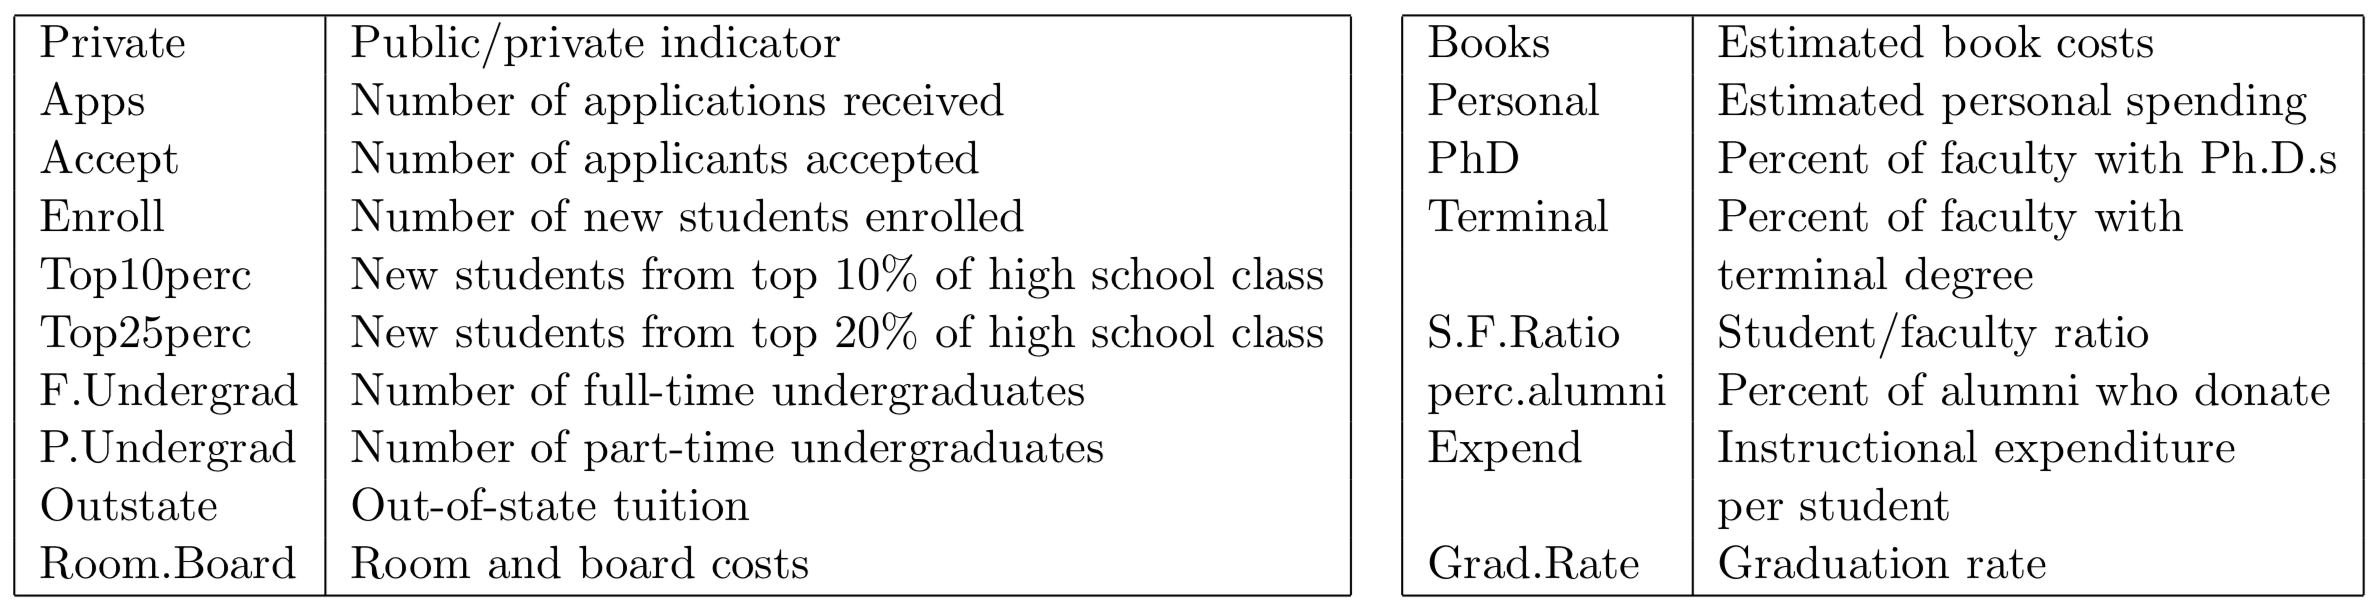
\includegraphics[width=\linewidth]{chart2.png}
	  \end{figure}
	    \begin{enumerate}
	      \item Read the data into R, for example, by the \textbf{load("College.rda")} and \textbf{attach("College.rda")} command. Make sure you have the directory set to the correct location for the data.
\begin{knitrout}
\definecolor{shadecolor}{rgb}{0.969, 0.969, 0.969}\color{fgcolor}\begin{kframe}
\begin{alltt}
\hlkwd{library}\hlstd{(ISLR)}
\hlkwd{attach}\hlstd{(College)}
\end{alltt}
\end{kframe}
\end{knitrout}
	      
	      \item Use the \textbf{summary()} function to produce a numerical summary of the variables in the data set.
\begin{knitrout}
\definecolor{shadecolor}{rgb}{0.969, 0.969, 0.969}\color{fgcolor}\begin{kframe}
\begin{alltt}
\hlkwd{summary}\hlstd{(College)}
\end{alltt}
\end{kframe}
\end{knitrout}
\begin{knitrout}
\definecolor{shadecolor}{rgb}{0.969, 0.969, 0.969}\color{fgcolor}\begin{kframe}
\begin{verbatim}
##  Private        Apps           Accept          Enroll       Top10perc    
##  No :212   Min.   :   81   Min.   :   72   Min.   :  35   Min.   : 1.00  
##  Yes:565   1st Qu.:  776   1st Qu.:  604   1st Qu.: 242   1st Qu.:15.00  
##            Median : 1558   Median : 1110   Median : 434   Median :23.00  
##            Mean   : 3002   Mean   : 2019   Mean   : 780   Mean   :27.56  
##            3rd Qu.: 3624   3rd Qu.: 2424   3rd Qu.: 902   3rd Qu.:35.00  
##            Max.   :48094   Max.   :26330   Max.   :6392   Max.   :96.00  
##    Top25perc      F.Undergrad     P.Undergrad         Outstate    
##  Min.   :  9.0   Min.   :  139   Min.   :    1.0   Min.   : 2340  
##  1st Qu.: 41.0   1st Qu.:  992   1st Qu.:   95.0   1st Qu.: 7320  
##  Median : 54.0   Median : 1707   Median :  353.0   Median : 9990  
##  Mean   : 55.8   Mean   : 3700   Mean   :  855.3   Mean   :10441  
##  3rd Qu.: 69.0   3rd Qu.: 4005   3rd Qu.:  967.0   3rd Qu.:12925  
##  Max.   :100.0   Max.   :31643   Max.   :21836.0   Max.   :21700  
##    Room.Board       Books           Personal         PhD        
##  Min.   :1780   Min.   :  96.0   Min.   : 250   Min.   :  8.00  
##  1st Qu.:3597   1st Qu.: 470.0   1st Qu.: 850   1st Qu.: 62.00  
##  Median :4200   Median : 500.0   Median :1200   Median : 75.00  
##  Mean   :4358   Mean   : 549.4   Mean   :1341   Mean   : 72.66  
##  3rd Qu.:5050   3rd Qu.: 600.0   3rd Qu.:1700   3rd Qu.: 85.00  
##  Max.   :8124   Max.   :2340.0   Max.   :6800   Max.   :103.00  
##     Terminal       S.F.Ratio      perc.alumni        Expend     
##  Min.   : 24.0   Min.   : 2.50   Min.   : 0.00   Min.   : 3186  
##  1st Qu.: 71.0   1st Qu.:11.50   1st Qu.:13.00   1st Qu.: 6751  
##  Median : 82.0   Median :13.60   Median :21.00   Median : 8377  
##  Mean   : 79.7   Mean   :14.09   Mean   :22.74   Mean   : 9660  
##  3rd Qu.: 92.0   3rd Qu.:16.50   3rd Qu.:31.00   3rd Qu.:10830  
##  Max.   :100.0   Max.   :39.80   Max.   :64.00   Max.   :56233  
##    Grad.Rate     
##  Min.   : 10.00  
##  1st Qu.: 53.00  
##  Median : 65.00  
##  Mean   : 65.46  
##  3rd Qu.: 78.00  
##  Max.   :118.00
\end{verbatim}
\end{kframe}
\end{knitrout}

	      \item Use the \textbf{pairs()} function to produce a scatterplot matrix of the first ten columns or variables of the data. Recall that you can reference the first ten columns of a matrix A using A[,1:10].
\begin{knitrout}
\definecolor{shadecolor}{rgb}{0.969, 0.969, 0.969}\color{fgcolor}\begin{kframe}
\begin{alltt}
\hlkwd{pairs}\hlstd{(College[,}\hlnum{1}\hlopt{:}\hlnum{10}\hlstd{])}
\end{alltt}
\end{kframe}
\end{knitrout}
\begin{knitrout}
\definecolor{shadecolor}{rgb}{0.969, 0.969, 0.969}\color{fgcolor}
\includegraphics[width=\maxwidth]{figure/4_cT-1} 

\end{knitrout}

	      \item Use the \textbf{plot()} function to produce side-by-side boxplots of Outstate versus Private.
\begin{knitrout}
\definecolor{shadecolor}{rgb}{0.969, 0.969, 0.969}\color{fgcolor}\begin{kframe}
\begin{alltt}
\hlkwd{plot}\hlstd{(Outstate}\hlopt{~}\hlstd{Private)}
\end{alltt}
\end{kframe}
\end{knitrout}
\begin{knitrout}
\definecolor{shadecolor}{rgb}{0.969, 0.969, 0.969}\color{fgcolor}
\includegraphics[width=4in,height=4in]{figure/4_dT-1} 

\end{knitrout}
	      \item Create a new qualitative variable, called \textbf{Elite}, by \textit{binning} the Top10perc variable. We are going to divide universities into two groups based on whether or not the proportion of students coming from the top 10\% of their high school classes exceeds 50\%:\\[1.5pt]
	      $>$ \textbf{Elite = rep ("No",nrow(College))}\\
        $>$ \textbf{Elite [College\$ Top10perc $>$ 50] = "Yes"}\\ 
        $>$ \textbf{Elite = as.factor (Elite)}\\
        $>$ \textbf{College = data.frame(College,Elite)}\\[1.5pt]
        Use the \textbf{summary()} function to see how many elite universities there are. Now use the \textbf{plot()} function to produce side-by-side boxplots of Outstate versus Elite.
\begin{knitrout}
\definecolor{shadecolor}{rgb}{0.969, 0.969, 0.969}\color{fgcolor}\begin{kframe}
\begin{alltt}
\hlstd{Elite} \hlkwb{=} \hlkwd{rep} \hlstd{(}\hlstr{"No"}\hlstd{,}\hlkwd{nrow}\hlstd{(College))}
\hlstd{Elite [College}\hlopt{$} \hlstd{Top10perc} \hlopt{>} \hlnum{50}\hlstd{]} \hlkwb{=} \hlstr{" Yes"}
\hlstd{Elite} \hlkwb{=} \hlkwd{as.factor} \hlstd{(Elite)}
\hlstd{College} \hlkwb{=} \hlkwd{data.frame}\hlstd{(College,Elite)}
\hlkwd{summary}\hlstd{(College}\hlopt{$}\hlstd{Elite)}
\end{alltt}
\end{kframe}
\end{knitrout}
\begin{knitrout}
\definecolor{shadecolor}{rgb}{0.969, 0.969, 0.969}\color{fgcolor}\begin{kframe}
\begin{verbatim}
##  Yes   No 
##   78  699
\end{verbatim}
\end{kframe}
\end{knitrout}
        \item Use the \textbf{hist()} function to produce some histograms with differing numbers of bins for a few of the quantitative variables. You may find the command \textbf{par(mfrow=c(2,2))} useful: it will divide the print window into four regions so that four plots can be made simultaneously. Modifying the arguments to this function will divide the screen in other ways.
\begin{knitrout}
\definecolor{shadecolor}{rgb}{0.969, 0.969, 0.969}\color{fgcolor}\begin{kframe}
\begin{alltt}
\hlkwd{par}\hlstd{(}\hlkwc{mfrow}\hlstd{=}\hlkwd{c}\hlstd{(}\hlnum{2}\hlstd{,}\hlnum{2}\hlstd{))}
\hlkwd{hist}\hlstd{(Books,} \hlkwc{breaks} \hlstd{=} \hlnum{10}\hlstd{)}
\hlkwd{hist}\hlstd{(Books,} \hlkwc{breaks} \hlstd{=} \hlnum{100}\hlstd{)}
\hlkwd{hist}\hlstd{(Apps,} \hlkwc{breaks} \hlstd{=} \hlnum{10}\hlstd{)}
\hlkwd{hist}\hlstd{(Apps,} \hlkwc{breaks} \hlstd{=} \hlnum{100}\hlstd{)}
\end{alltt}
\end{kframe}
\end{knitrout}
\begin{knitrout}
\definecolor{shadecolor}{rgb}{0.969, 0.969, 0.969}\color{fgcolor}
\includegraphics[width=\maxwidth]{figure/4_fT-1} 

\end{knitrout}

        \item Use the \textbf{lm} function to find a regression equation predicting the number of new students based on the graduation rate, qualifications of the faculty, and various expenses.
\begin{knitrout}
\definecolor{shadecolor}{rgb}{0.969, 0.969, 0.969}\color{fgcolor}\begin{kframe}
\begin{alltt}
\hlkwd{lm}\hlstd{(Enroll} \hlopt{~} \hlstd{Grad.Rate} \hlopt{+} \hlstd{Terminal} \hlopt{+} \hlstd{PhD} \hlopt{+}
     \hlstd{Expend} \hlopt{+} \hlstd{Personal} \hlopt{+} \hlstd{Books} \hlopt{+} \hlstd{Room.Board} \hlopt{+} \hlstd{Outstate)}
\end{alltt}
\end{kframe}
\end{knitrout}
\begin{knitrout}
\definecolor{shadecolor}{rgb}{0.969, 0.969, 0.969}\color{fgcolor}\begin{kframe}
\begin{verbatim}
## 
## Call:
## lm(formula = Enroll ~ Grad.Rate + Terminal + PhD + Expend + Personal + 
##     Books + Room.Board + Outstate)
## 
## Coefficients:
## (Intercept)    Grad.Rate     Terminal          PhD       Expend  
##  -1.236e+03    4.282e+00    1.084e+01    1.476e+01    2.254e-02  
##    Personal        Books   Room.Board     Outstate  
##   2.657e-01    3.038e-01    8.804e-03   -9.386e-02
\end{verbatim}
\end{kframe}
\end{knitrout}
	    \end{enumerate}
	\end{problem}
% 5.	
	\begin{problem} (\#3-6, page 121). Argue that in the case of simple linear regression, the least squares line always passes through the point of averages ($\bar{X}$, $\bar{Y}$).\\[5pt]
	SLR: $\hat{Y_i} = \hat{\beta_0} + \hat{\beta_1}X_i$, we know that $\hat{\beta_0} = \bar{Y} - \hat{\beta_1}\bar{X}$, when $X_i = \bar{X}$,
	$$\hat{Y} = (\bar{Y} - \hat{\beta_1}\bar{X}) + \hat{\beta_1}\bar{X} = \bar{Y}$$
	So, the SLR line passes throught ($\bar{X}$, $\bar{Y}$).
	\end{problem}
\end{document}
